\documentclass{beamer}
\usetheme{Boadilla}
\usepackage{hyperref}
\usepackage{graphicx}
\usepackage{fancyvrb}
\usepackage{multicol}
\usepackage{adjustbox}
\usepackage{tikz}
\usetikzlibrary{shapes,positioning}
\newcommand{\foo}{\hspace{-2.3pt}$\bullet$ \hspace{5pt}}
\usepackage{subfig}
\usepackage[
    backend=biber, 
    natbib=true,
    style=numeric,
    sorting=none,
    style=verbose-ibid,
]{biblatex}
\addbibresource{citations.bib}
\usepackage{pgfpages}
\usepackage{xcolor}
\definecolor{ao(english)}{rgb}{0.0, 0.5, 0.0}
\definecolor{burgundy}{rgb}{0.5, 0.0, 0.13}
%\setbeameroption{show notes}
\setbeameroption{show notes on second screen=right}
%\setbeameroption{hide notes}

\title{Dynamic Programming for Beat Tracking}
\author{Sevag Hanssian}
\date{Feburary 16, 2021}
\institute{MUMT 621, Winter 2021}
\setbeamertemplate{navigation symbols}{}

\begin{document}

\begin{frame}
\maketitle
\end{frame}

\begin{frame}
	\frametitle{Dynamic programming}
	hello \footfullcite{opuspaper}
	\begin{figure}
	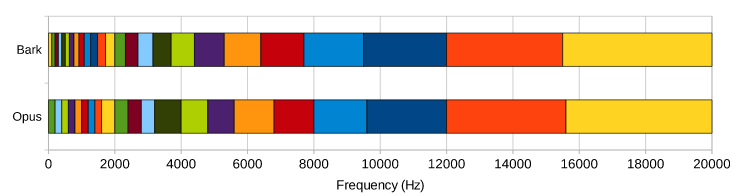
\includegraphics[width=8cm]{./bark.png}
	\end{figure}
\end{frame}

\note{
	\begin{itemize}
		\item
			like lpc is dominant for speech, mdct is dominant for audio codecs
		\item
			lots of DCTs, details were too much to get into
		\item
			fewer coefficients means that the DCT is very used in compression
	\end{itemize}
}

\end{document}
